\documentclass[dvipdfmx,journal]{IEEEtran}

\usepackage[ruled, vlined]{algorithm2e}    % \begin{algorithm2e}
\usepackage{amsmath}        % \begin{align*}
\usepackage{amssymb}        % \mathbb{A}
\usepackage{amsthm}         % \newtheorem
\usepackage{bm,bbm}         % \bm{A}, \bbm{1}
\usepackage{booktabs}       % \toprule, \midrule, \bottomrule
\usepackage{caption}        % \captionsetup
\usepackage{enumitem}       % \begin{enumerate}[label=(\alph*)]
\usepackage[dvipdfmx]{hyperref}       % \href{URL}{text}
\usepackage{ifthen}         % \ifthenelse
\usepackage{lipsum}         % \lipsum
\usepackage{mathrsfs}       % \mathscr{A}
\usepackage{mathtools}      % \mathrlap
\usepackage{optidef}        % \begin{mini*}{x}{f(x)}{}{}
\usepackage{orcidlink}      % \orcidlink
\usepackage{physics}        % \qty, \norm, \abs
\usepackage{subfiles}       % \subfile{file}
\usepackage{thm-restate}    % \begin{restatable}{theorem}{thm}
\usepackage{tikz}           % \begin{tikzpicture}
\usepackage{xparse}         % \NewDocumentCommand
% \usepackage{calc}         % \setlength
% \usepackage{cancel}       % \cancel
% \usepackage{parskip}      % \setlength{\parskip}{0.5em}
% \usepackage{csvsimple}    % \csvautotabular
% \usepackage{diagbox}      % \diagbox
% \usepackage{dsfont}       % \mathds{1}
% \usepackage{epsfig}       % \epsfig
% \usepackage{fancybx}      % \ovalbox
% \usepackage{float}        % \begin{figure}[H]
% \usepackage{lipsum}       % \lipsum
% \usepackage{listings}     % \begin{lstlisting}
% \usepackage{makecell}     % \makecell{L1\L2}
% \usepackage{multicol}     % \begin{multicols}{2}
% \usepackage{multirow}     % \multirow
% \usepackage{nicematrix}   % \begin{NiceMatrix}
% \usepackage{qcircuit}     % \Qcircuit
% \usepackage{siunitx}      % \SI{1}{\second}
% \usepackage{stfloats}     % \begin{figure*}
% \usepackage{subcaption}   % \begin{subfigure}
% \usepackage{ulem}         % \sout
% \usepackage{wrapfig}      % \begin{wrapfigure}
% \usepackage[all]{xy}      % \xymatrix
% \usepackage[dvipdfmx]{graphicx}
% \usepackage[square, sort, comma, numbers]{natbib}

\hypersetup{colorlinks=true,linkcolor=blue,citecolor=blue,urlcolor=blue}

\definecolor{cA}{HTML}{0072BD}
\definecolor{cB}{HTML}{EDB120}
\definecolor{cC}{HTML}{77AC30}
\definecolor{cD}{HTML}{D95319}

\newcommand{\red}[1]{\textcolor{red}{#1}}
\newcommand{\blue}[1]{\textcolor{blue}{#1}}
\newcommand{\cyan}[1]{\textcolor{cyan}{#1}}
\newcommand{\gray}[1]{\textcolor{gray}{#1}}
\newcommand{\green}[1]{\textcolor{green}{#1}}
\newcommand{\brown}[1]{\textcolor{brown}{#1}}
\newcommand{\black}[1]{\textcolor{black}{#1}}
\newcommand{\orange}[1]{\textcolor{orange}{#1}}
\newcommand{\st}{\text{ s.t. }}
\newcommand{\Img}[1]{\mathrm{Im}\qty(#1)}
\newcommand{\Ker}[1]{\mathrm{Ker}\qty(#1)}
\newcommand{\Supp}[1]{\mathrm{supp}\qty(#1)}
\newcommand{\Rank}[1]{\mathrm{rank}\qty(#1)}
\newcommand{\floor}[1]{\left\lfloor #1 \right\rfloor}
\newcommand{\ceil}[1]{\left\lceil #1 \right\rceil}
% C++ (https://tex.stackexchange.com/questions/4302/prettiest-way-to-typeset-c-cplusplus)
\newcommand{\Cpp}{C\nolinebreak[4]\hspace{-.05em}\raisebox{.4ex}{\relsize{-3}{\textbf{++}}}}
% https://tex.stackexchange.com/questions/28836/typesetting-the-define-equals-symbol
\newcommand{\defeq}{\coloneqq}
\newcommand{\eqdef}{\eqqcolon}
% https://tex.stackexchange.com/questions/5502/how-to-get-a-mid-binary-relation-that-grows
\newcommand{\relmiddle}[1]{\mathrel{}\middle#1\mathrel{}}

% https://tex.stackexchange.com/questions/564216/newcommand-for-each-letter
\ExplSyntaxOn
\NewDocumentCommand{\definealphabet}{mmmm}{
\int_step_inline:nnn{`#3}{`#4}{
\cs_new_protected:cpx{#1 \char_generate:nn{##1}{11}}{
\exp_not:N #2{\char_generate:nn{##1}{11}}}}}
\ExplSyntaxOff

\definealphabet{bb}{\mathbb}{A}{Z}
\definealphabet{rm}{\mathrm}{A}{Z}
\definealphabet{cal}{\mathcal}{A}{Z}
\definealphabet{frak}{\mathfrak}{a}{z}
% \definealphabet{scr}{\mathscr}{A}{Z}
% \definealphabet{frak}{\mathfrak}{A}{Z}

\newtheorem{theorem}{Theorem}
\newtheorem{proposition}{Proposition}
\newtheorem{lemma}{Lemma}
\newtheorem{definition}{Definition}
\newtheorem{corollary}{Corollary}
\newtheorem{remark}{Remark}
\newtheorem{example}{Example}
\newtheorem{assumption}{Assumption}

% https://qiita.com/rityo_masu/items/efd44bc8f9229e014237
\allowdisplaybreaks[4]

\usetikzlibrary{
  3d,
  % fit,
  calc,
  math,
  matrix,
  patterns,
  backgrounds,
  arrows.meta,
  shapes.geometric,
  decorations.pathmorphing,
}


% \providecommand{\main}{.}
\newboolean{isMain}
\setboolean{isMain}{true}

\begin{document}
\bstctlcite{IEEEexample:BSTcontrol}

\title{Fruchterman--Reingold Layout with\\Subspace Method as Initial Placement}
\author{
  \orcidlinki{Hiroki Hamaguchi}{0009-0005-7348-1356} % TODO: fix
  \orcidlinki{Naoki Marumo}{0000-0002-7372-4275} % ? maybe dvipdfmx problem
  Akiko Takeda
  \thanks{
    We all are with Graduate School of Information Science and Technology, The University of Tokyo, Tokyo, Japan. A. Takeda is with Center for Advanced Intelligence Project, RIKEN, Tokyo, Japan.
  }
}
\date{\today}
\maketitle

\begin{abstract}
  The abstract goes here.
  \lipsum[1]
\end{abstract}

\begin{IEEEkeywords}
  Graph drawing, Fruchterman--Reingold algorithm, Random Subspace method.
\end{IEEEkeywords}

\section{Introduction}\label{sec:introduction}

\IEEEPARstart{G}{raph} is a mathematical structure representing pairwise relationships between objects, and graph drawing is one of the most fundamental tasks in data science. Indeed, Numerous general algorithms have been proposed for graph drawing~\cite{tutteHowDrawGraph1963,chrobakLineartimeAlgorithmDrawing1995,sugiyamaMethodsVisualUnderstanding1981,ghassemitoosiSimulatedAnnealingPreProcessing2016}
Among these, one of the most popular strategies is force-directed algorithms.

In force-directed algorithms, the graph is modeled as a physical system of particles. These include methods such as the Kamada--Kawai (KK) layout~\cite{kamadaAlgorithmDrawingGeneral1989} using shortest path distances for a cost function, and the Fruchterman--Reingold (FR) layout~\cite{fruchtermanGraphDrawingForcedirected1991,kobourovSpringEmbeddersForce2012}, which is the primary focus of this paper.

The FR algorithm is one of the most widely used force-directed algorithms. It is also implemented in many modern graph drawing libraries such as NetworkX~\cite{osti_960616}, Graphviz~\cite{ellsonGraphvizOpenSource2002}, and igraph~\cite{csardiIgraphSoftwarePackage2006}. The FR layout is based on a physical model of a system of particles and springs, and FR algorithm seeks the equilibrium of the forces between nodes.

However, since both the KK layout and the FR layout requires to compute the forces or energies between all pairs of vertices, they have a high computational cost of $\order{n^2}$ per iteration, where $n$ is the number of vertices in the graph. To address this kind of computational burden, several methods have been proposed. One strategy is to approximate the $n$-body simulation using hierarchical methods such as the fast multipole method~\cite{greengardFastAlgorithmParticle1987}, the Barnes--Hut approximation~\cite{barnesHierarchicalLogForcecalculation1986}, multilevel approaches~\cite{Hu2006EfficientHF}, or stress majorization~\cite{gansnerGraphDrawingStress2005}.

Another approach is to accelerate the optimization algorithm directly, which aligns with the spirit of our work. Recent researches have accelerated the algorithms for FR layout and KK layout through various methods, including GPU parallel architectures~\cite{gajdosParallelFruchtermanReingold2016}, numerical optimization techniques such as L-BFGS~\cite{6183577}, and Stochastic Gradient Descent (SGD)~\cite{8419285}.

Based on such advances, in this paper, we investigate the ability of another algorithm: subspace methods.

\begin{figure}[t]
  \centering
  \begin{tabular}{cc}
    \large{\textbf{FR}}                                          & \large{\textbf{L-BFGS}}   \\
    \begin{minipage}{0.45\columnwidth}
      \centering
      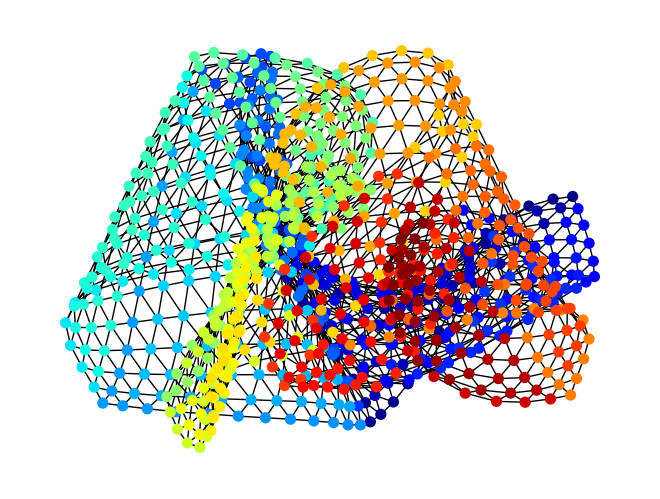
\includegraphics[width=\columnwidth]{jagmesh1_FR_50iter.png}
    \end{minipage} &
    \begin{minipage}{0.45\columnwidth}
      \centering
      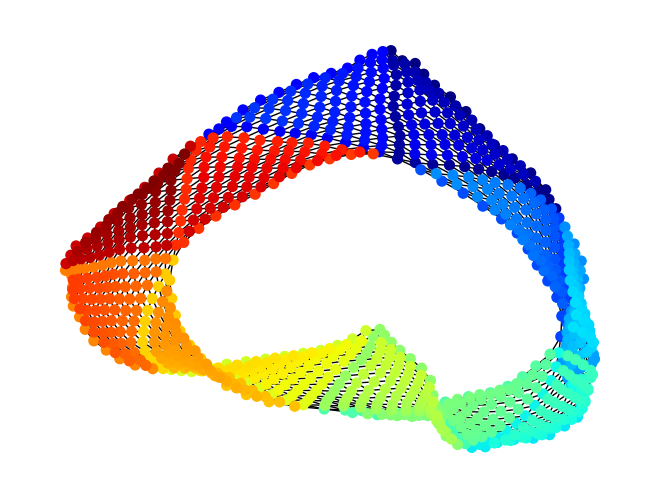
\includegraphics[width=\columnwidth]{jagmesh1_LBFGS_50iter.png}
    \end{minipage}                           \\
    \large{\textbf{proposed}}                                    & \large{\textbf{+ L-BFGS}} \\
    \begin{minipage}{0.45\columnwidth}
      \centering
      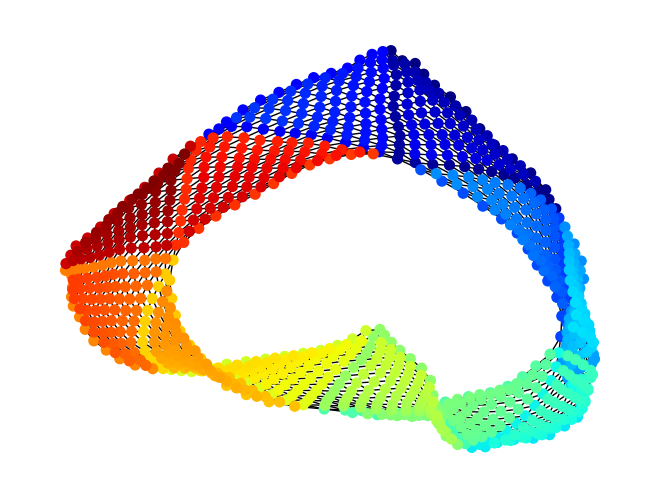
\includegraphics[width=\columnwidth]{jagmesh1_LBFGS_50iter.png}
    \end{minipage}
                                                                 &
    \begin{minipage}{0.45\columnwidth}
      \centering
      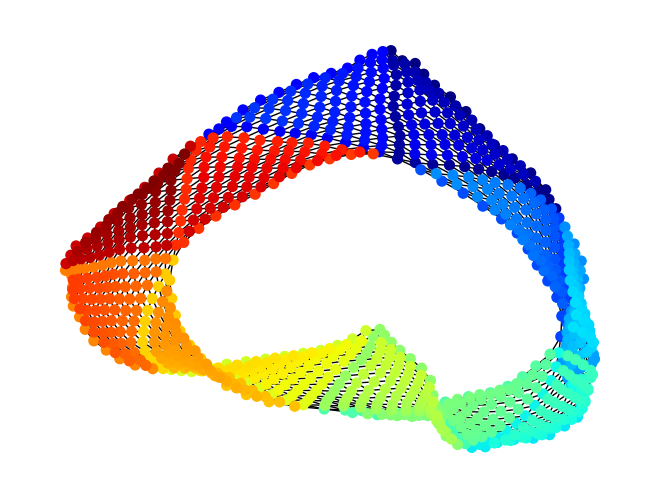
\includegraphics[width=\columnwidth]{jagmesh1_LBFGS_50iter.png}
    \end{minipage}
  \end{tabular}
  \begin{tikzpicture}[overlay, remember picture]
    \draw[->, thick] (-0.3,1.3) -- (+0.3,1.3);
  \end{tikzpicture}
  \caption{
    Comparison of the FR algorithm, L-BFGS, and the proposed method
    for the \texttt{jagmesh1} dataset.}
  \label{table:four_images}
\end{figure}

The rest of the paper is organized as follows.
In Section~\ref{sec:preliminary}, we define the optimization problem for the FR algorithm.
In Section~\ref{sec:RQ}, we present our research question based on previous works.
In Section~\ref{sec:algorithm}, we propose a new algorithm that utilizes the subspace method for the FR layout.
In Section~\ref{sec:experiment}, we present our experimental results.
Finally, we conclude and discuss future work in Section~\ref{sec:discussion}.

\section{Preliminary}\label{sec:preliminary}

\begin{figure}[t]
  \centering
  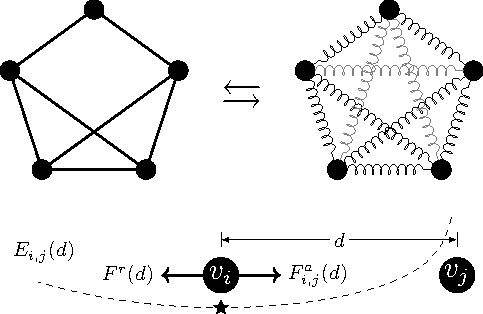
\includegraphics[height=5.5cm]{fr_layout.pdf}
  \caption{
    (Top) Fruchterman--Reingold layout. It models $\order{n^2}$ springs between all pairs of vertices.
    (Bottom) The equilibrium between attractive force $F_{i,j}^a(d)$ and repulsive force $F^r(d)$ is achieved at $d = k/\sqrt[3]{w_{i,j}}$, which equals $k$ when $w_{i,j} = 1$.
  }
  \label{fig:frLayout}
\end{figure}

Firstly, in this section, we formulate the FR layout as a continuous optimization problem, and introduce the conventional approaches to this problem, namely the FR algorithm and the L-BFGS method.

\subsection{Fruchterman--Reingold layout}\label{ssec:frLayout}

Let us define
$\bbR_{> 0} \defeq \qty{ x \in \bbR \mid x > 0 }, \quad \bbR_{\geq 0} \defeq \qty{ x \in \bbR \mid x \geq 0 }$,
and let $W = (w_{i,j}) \in \bbR_{\geq 0}^{n \times n}$ be an adjacency matrix of a undirected connected graph $G_W = (V, E)$. $V = \qty{v_i \mid 1 \leq i \leq n}$ is a set of vertices and $E = \qty{(v_i, v_j) \mid w_{i,j} > 0}$ is a set of edges. We call $w_{i,j}$ as a weight of the edge $(v_i, v_j)$.

The FR algorithm in NetworkX, for example, can handle directed unconnected graphs with $w_{i,j} < 0$, but we will not consider such cases here.
For directed graphs, slight modifications of algorithms or converting them to undirected graphs may be effective. For unconnected graphs, algorithms can be applied to each connected component independently. When $w_{i,j} < 0$ for some $(i,j)$, the optimization problem may become unbounded, but with $w_{i,j} \geq 0$ for all $(i,j)$ and the connectivity, the problem is always bounded and solvable.

In summary, the conditions for $W$ is formulated as follows:
\begin{equation}\label{eq:WCondition}
  W \in \bbR_{\geq 0}^{n \times n}, \quad W = W^\top, \quad \text{$G_W$ is connected}.
\end{equation}

Each vertex $v_i \in V$ is assigned to a point on a plane $x_i \in \bbR^2$ and we define $X = (x_1, \dots, x_n) \in \bbR^{2 \times n}$ as the configuration of the graph.
For an parameter $k$ and a distance $d_{i,j} \defeq \norm{x_i - x_j}_2$ between two vertices $v_i$ and $v_j$, Fruchterman and Reingold~\cite{fruchtermanGraphDrawingForcedirected1991} defined the power of attraction $F_{i,j}^a: \bbR_{> 0} \to \bbR$ and the power of repulsion $F^r: \bbR_{> 0} \to \bbR$ as
\begin{equation*}
  F_{i,j}^a(d) \defeq \frac{w_{i,j} d^2}{k}, \quad F^r(d) \defeq -\frac{k^2}{d}.
\end{equation*}
We refer this force-directed layout as the Fruchterman--Reingold (FR) layout.
The energy for these powers $E_{i,j}(d)$ can be defined as
\begin{align*}
  E_{i,j}(d) & \defeq \int_{0}^{d} F_{i,j}^a(r) \dd{r} + \int_{\infty}^{d} F^r(r) \dd{r} \\
             & = \frac{w_{i,j} d^3}{3k} - k^2\log{d}.
\end{align*}
As a remark, the energy function $E_{i,j}$ is convex as a function of $d$ and minimized when $d^* = k/\sqrt[3]{w_{i,j}}$, but it is not Lipschitz continuous, and is not convex as a function of $x_i$. Refer to Figure~\ref{fig:energy3d}.

\begin{figure}[t]
  \centering
  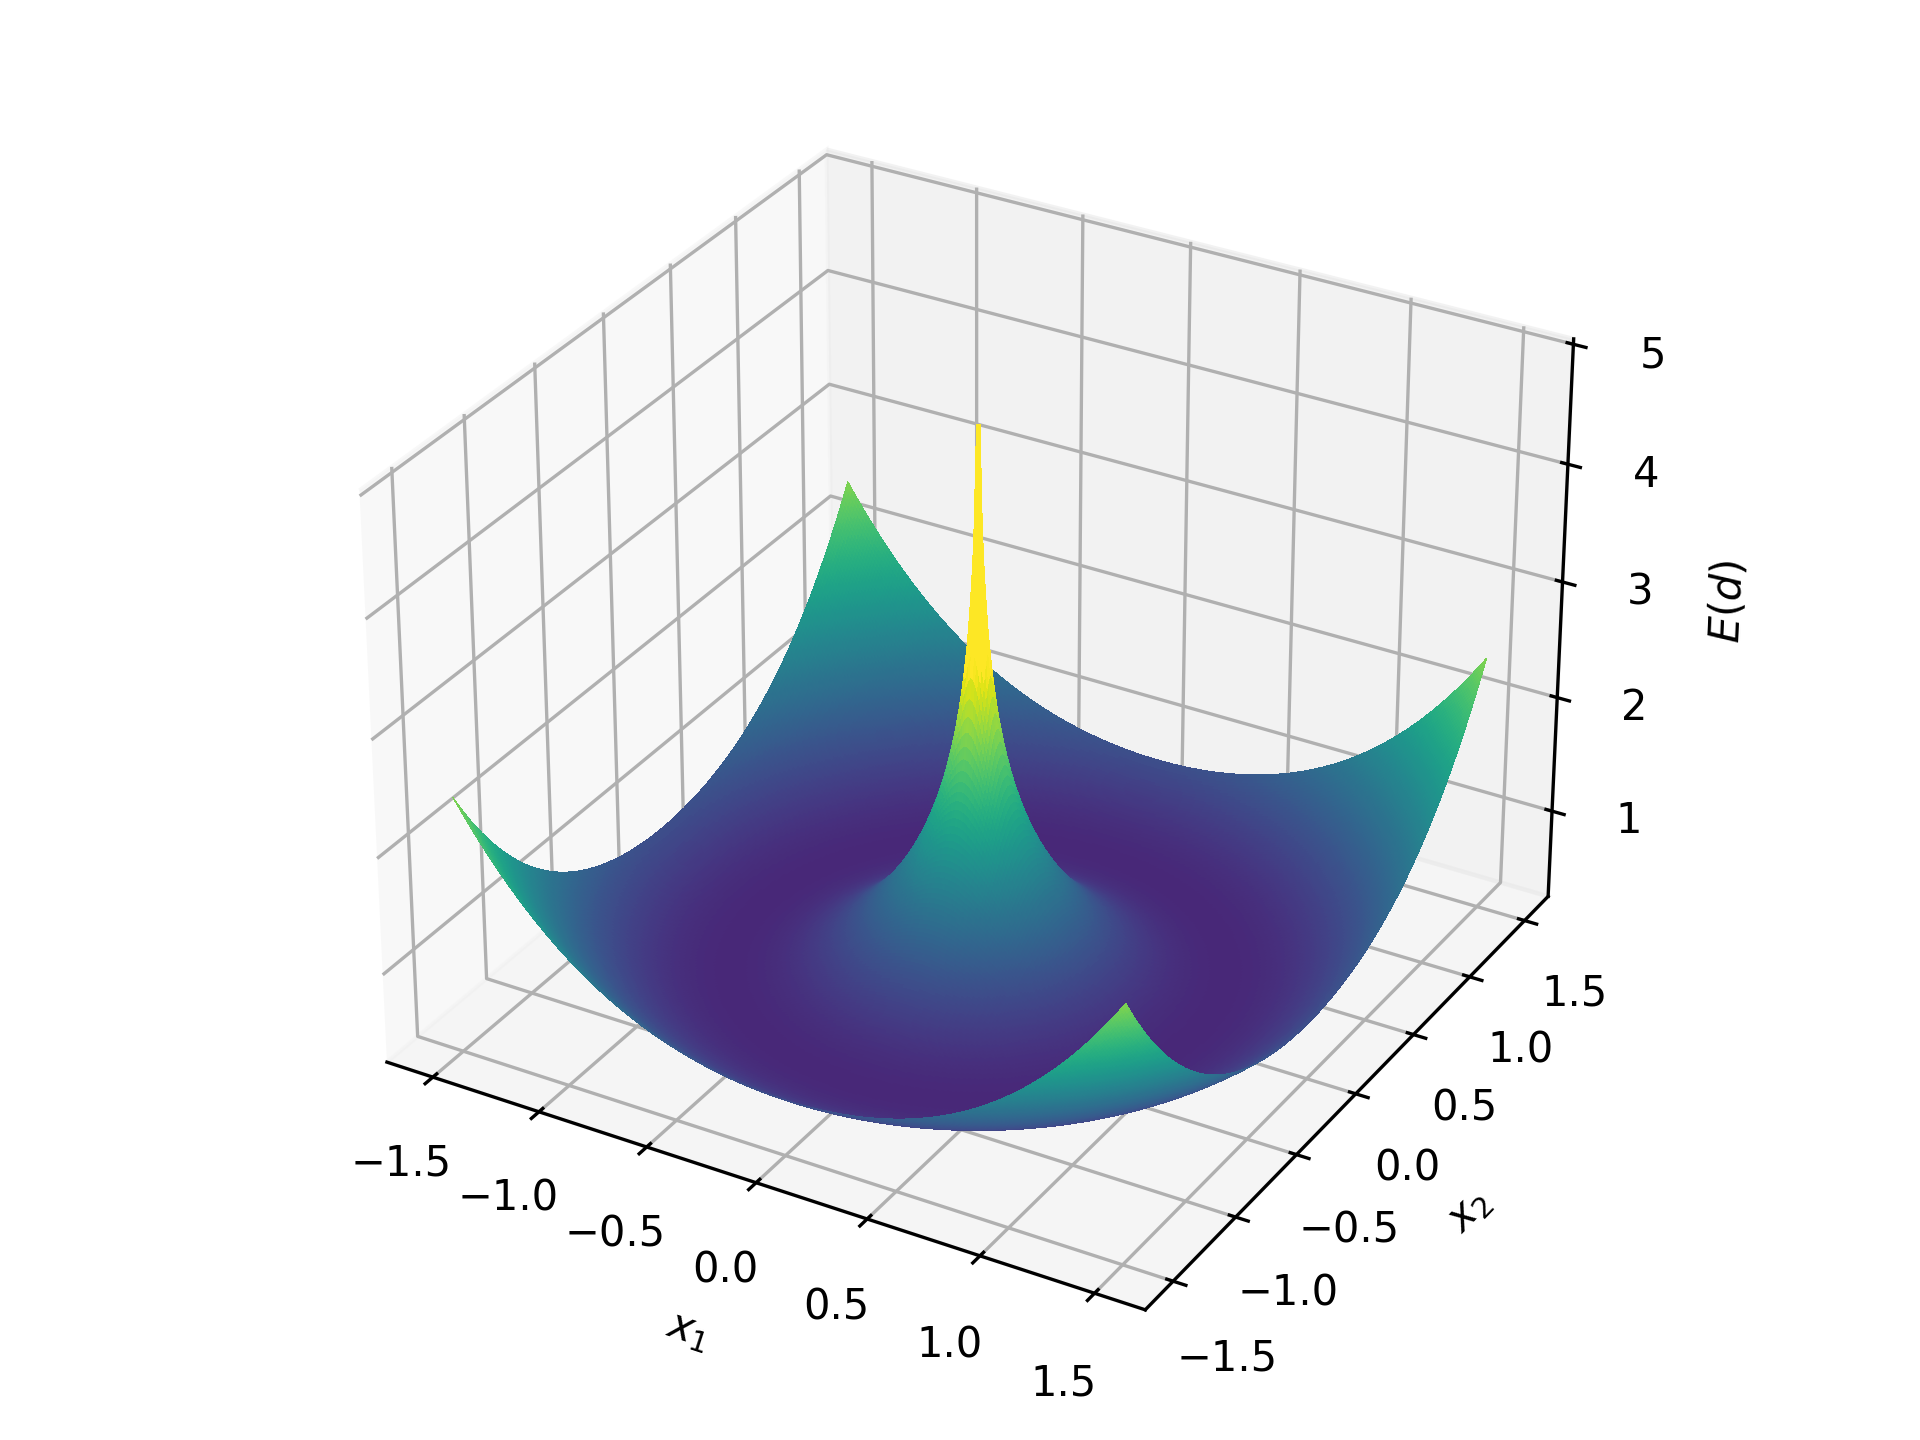
\includegraphics[height=5.5cm]{energy_3d.png}
  \caption{Energy function $E_{i,j}(d)$ for $x_j=(0,0)$, $w_{i,j} = 1$ and $k = 1$. Although $E_{i,j}$ is convex as a function of $d$, it is not convex as a function of $x_i$. As $x_i$ approaches $x_j$, the energy function diverges.}
  \label{fig:energy3d}
\end{figure}

Now, the optimization problem for FR layout can be formulated as the minimization of the energy function $f: \bbR^{2 \times n} \to \bbR$, as known as a stress of the graph:
\begin{mini}
  {X \in \bbR^{2 \times n}}
  {f(X) \defeq \sum_{i<j} E_{i,j}(d_{i,j})}
  {\label{eq:fr}}
  {}
\end{mini}
In the following, we will discuss the optimization of this problem.

\begin{figure*}[t]
  \begin{minipage}{0.49\hsize}
    \centering
    \begin{tabular}{ccc}
      \texttt{sfdp}                                             & \texttt{fdp} & \texttt{spring\_layout} \\
      
\includegraphics[width=0.27\columnwidth]{circle_sfdp.png} &
      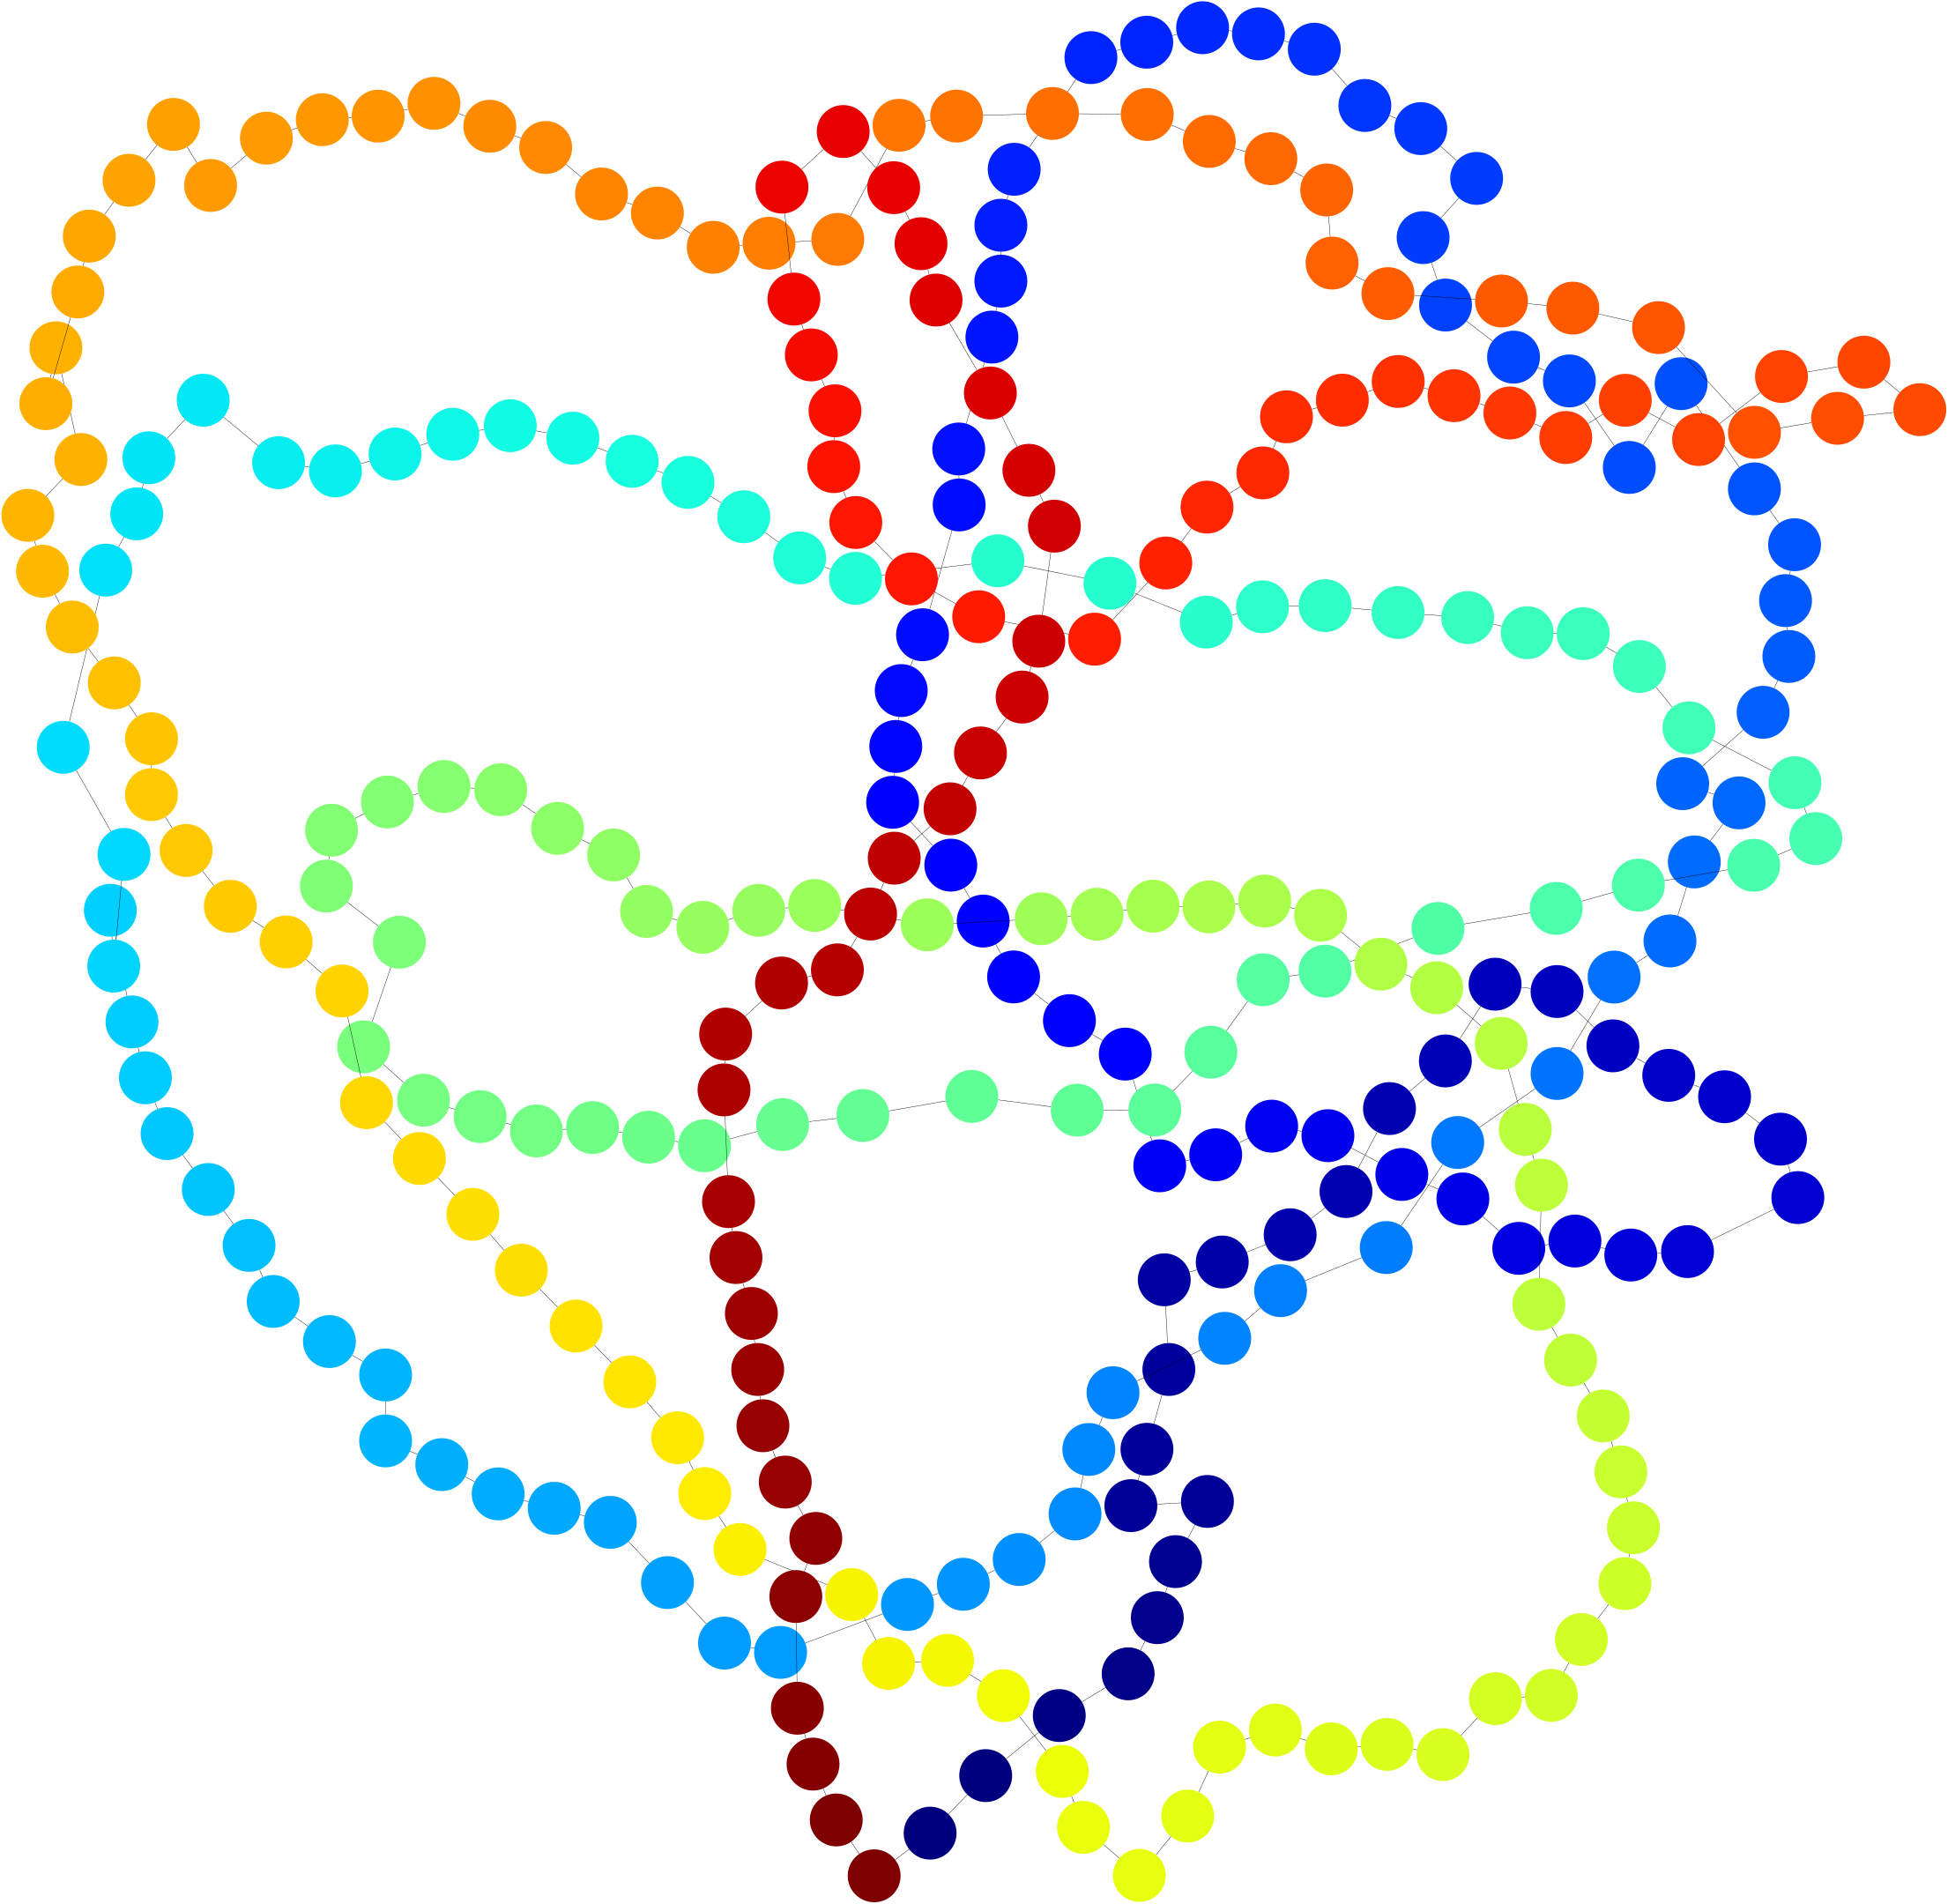
\includegraphics[width=0.27\columnwidth]{circle_fdp.png}  &
      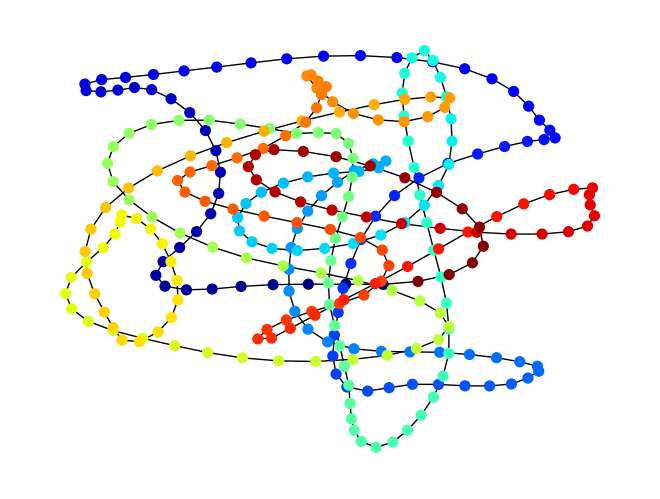
\includegraphics[width=0.27\columnwidth]{circle_fr.png}                                            \\
    \end{tabular}
    \caption{
      Comparison of \texttt{sfdp} in Graphviz, \texttt{fdp} in Graphviz, and \texttt{spring\_layout} in NetworkX for the circle graph with $\abs{V} = 300$.
      Every algorithm is run with the default parameters, but both \texttt{fdp} and \texttt{spring\_layout} fails to beautifully visualize the circle.
    }
    \label{fig:circle}
  \end{minipage}
  \begin{minipage}{0.49\hsize}
    \centering
    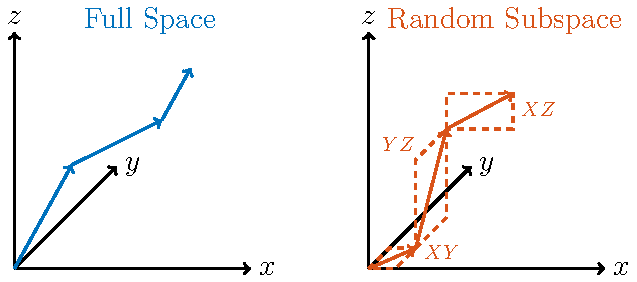
\includegraphics[width=\columnwidth]{randomSubspace.pdf}
    \caption{
      Visual explanation of Random Subspace Newton
      \orange{TODO}
    }
  \end{minipage}
\end{figure*}

\subsection{Fruchterman--Reingold algorithm}\label{ssec:frAlgorithm}

The Fruchterman--Reingold algorithm~\cite{fruchtermanGraphDrawingForcedirected1991}, the original force-directed algorithm for this layout, can be regarded as a most standard approach to solve the optimization problem~\eqref{eq:fr}.
As pointed out in~\cite{tunkelang1999numerical}, the FR algorithm can be regarded as a gradient descent method for the energy function $f$ with a cooling global temperature $t$.

Let denote $f_i(x): \bbR^2 \to \bbR$ as the energy function for the vertex $v_i$:
\begin{equation*}
  f_i(x_i) \defeq \sum_{j \neq i} E_{i,j}(d_{i,j}).
\end{equation*}
The gradient of $f_i$ is
\begin{equation}\label{eq:gradientFi}
  \nabla f_i(x_i) = \sum_{j \neq i} \qty(\frac{w_{i,j}d_{i,j}}{k} - \frac{k^2}{d_{i,j}^2}) (x_i-x_j),
\end{equation}
which is the sum of forces acting on the vertex $v_i$.

The pseudo code of the FR algorithm is shown in Algorithm~\ref{alg:fr}. It is based on the original implementation in~\cite{fruchtermanGraphDrawingForcedirected1991} and implementation in NetworkX~\cite{osti_960616} with some omitted details.

\begin{algorithm}[ht]
  \caption{Fruchterman--Reingold algorithm}
  \label{alg:fr}
  \KwIn{Graph $G_W = (V, E)$}
  \KwOut{Point configuration $X = (x_1, \dots, x_n)$}

  $\text{define parameters } k, t, dt, \text{iterations}$\;
  $x_i \gets \text{random}$ for all $v_i \in V$\;
  \For{$j \gets 0$ \KwTo \textit{iterations}}{
    $\text{compute gradient } \nabla f_i(x_i)$ for all $v_i \in V$\;
    $x_i \gets x_i + t \frac{\nabla f_i(x_i)}{
        \norm{\nabla f_i(x_i)}_{2}}$ for all $v_i \in V$\;
    $t \gets t - dt$\;
    \If{\text{convergence condition}}{
      \textbf{break}\;
    }
  }
  \Return $\text{pos}$
\end{algorithm}

In Algorithm~\ref{alg:fr}, the initial placement of points is determined randomly. In general, under proper normalization of the input, each point is uniformly distributed within a unit square.
The parameter $t$ denotes the temperature, which governs the step size of the gradient descent. As the temperature gradually decreases, the algorithm converges to a particular configuration, though this configuration is not necessarily the optimal solution.

\subsection{L-BFGS method}\label{ssec:lbfgs}

Another approach to solve the optimization problem~\eqref{eq:fr} is to use the Limited-memory Broyden--Fletcher--Goldfarb--Shanno (L-BFGS) algorithm~\cite{6183577}.
The L-BFGS method is an optimization technique used for large-scale problems, which approximates the inverse Hessian matrix using only a few recent gradient vectors, making it more memory-efficient than the standard BFGS method~\cite{liuLimitedMemoryBFGS1989}.
This makes L-BFGS particularly suitable for high-dimensional optimization tasks, and since it is a sophisticated method than the gradient descent method, the superior performance than the FR algorithm is reported in~\cite{6183577}.

There are many implementations of L-BFGS available, such as SciPy~\cite{2020SciPy-NMeth} and C++ L-BFGS~\cite{qiuYixuanLBFGSpp2024,okazakiChokkanLiblbfgs2024}.

For the optimization problem~\eqref{eq:fr}, the L-BFGS method can be applied via flattening the configuration $X \in \bbR^{2 \times n}$ to a vector $\overline{X} \in \bbR^{2n}$.
However, it is worth noting that this method ignores the structure of $X$, and treats the problem just as a general optimization problem. Thus, we can expect that there could be a room for improvement by leveraging what we have ignored in this L-BFGS method.

\section{Research Question}\label{sec:RQ}

Now, we declare the research question of this paper: ``Can we accelerate the optimization process for the FR layout by leveraging the inherent structure of the problem?''.

In the previous section, we presented the FR algorithm and L-BFGS method.
However, both methods face specific challenges during optimization, leading to inefficiencies and slow convergence as detailed in Section~\ref{ssec:twist}.
Addressing these challenges forms a part of our research question, and we aim to introduce a new algorithm capable of overcoming these limitations. To achieve this, we will review key prior studies in Sections~\ref{ssec:sgd} and~\ref{ssec:introRSN}.

\subsection{ねじれの発生}\label{ssec:twist}

いくつかの実験及び先行研究の報告を基にすると、FR layoutに対する最適化を考える上での最大の難点は、"ねじれ"の解消であると我々は考えている。

ねじれという言葉の用法自体は比較的少ないと認識しているが、例えば\cite{cheongSnapshotVisualizationComplex2018}などでもこの言葉が用いられている。本論文におけるねじれとは、数学的に厳密な語ではなく、図示した際に現れる明らかに不必要な線分の交差や、本来円環状などの簡潔な構造が絡まっているように見える状況を指している。
図~\ref{fig:circle}などに示したような状況が具体例である。

これがもし、グニャグニャに曲がっているが辺同士の交差が一切ない状況にある場合、FR algorithmやL-BFGS methodによる最適化は比較的速やかに進んでいく。しかし、そうでない場合、勾配が小さくなってしまい、通常の連続最適化では停滞してしまい、その解消は難しい。

故に、あらかじめできる限りねじれを解消するような初期配置を与えることは、最適化の効率に大きく影響を及ぼしうると考えられる。

\subsection{SGD for KK layout}\label{ssec:sgd}

Moreover, the effectiveness of Stochastic Gradient Descent (SGD) for Kama--Kawai (KK) layout is well-documented in~\cite{8419285}.
The KK layout is a energy based layout, which minimize the energy function $f^{\mathrm{KK}}$ defined as
\begin{equation*}
  f^{\mathrm{KK}}(X) = \sum_{i<j} f^{\mathrm{KK}}_{i,j}(d_{i,j}) = \sum_{i<j} \frac{k}{2}(d_{i,j}-l_{i,j})^2,
\end{equation*}
where $k$ is a constant, and $l_{i,j}$ is the optimal distance between them calculated from the shortest path distance in the graph.
The SGD method randomly selects pairs of vertices $(i,j)$ and adjusts their positions to minimize $f^{\mathrm{KK}}_{i,j}$ along the gradient direction, i.e. $x_i \gets x_i - \eta \nabla f^{\mathrm{KK}}_{i,j}(d_{i,j})$ and $x_j \gets x_j + \eta \nabla f^{\mathrm{KK}}_{i,j}(d_{i,j})$ with a learning rate $\eta$.

However, in contrast to the KK layout, the FR layout assigns the function $-k^2\log{d_{i,j}}$ to all $(i,j) \notin E$, making SGD relatively less effective for the FR layout.
Though, the superiority of SGD in the KK layout, which focuses on randomly selected edge, suggests that an optimization method focuses on randomly selected vertex may also be effective in the FR layout.
This observation motivates us to explore the application of Random Subspace Newton (RSN) to the FR layout as discussed in the next subsection.

\subsection{Introduction of Random Subspace Newton}\label{ssec:introRSN}

Now, we introduce the RSN method, which is not a proposed method itself, but a concept that heavily inspired our proposed algorithm.
The RSN method and its variant have been proposed in the context of optimization problems~\cite{NEURIPS2019_bc6dc48b,fujiRandomizedSubspaceRegularized2022,cartisRandomisedSubspaceMethods2022,higuchiFastConvergenceSecondOrder2024}.

RSN is a variant of the Newton's method. For a convex function $f(x): \bbR^n \to \bbR$, the Newton's method updates by $x \gets x - \nabla^2 f(x)^{-1} \nabla f(x)$.
This requires to compute the inverse of Hessian matrix $\nabla^2 f(x)^{-1} \in \bbR^{n \times n}$ at each iteration, which poses a high computational cost for large-scale problems.
In contrast, RSN focuses on a subspace of dimension $s$ randomly selected from the solution space by a projection matrix $P$ and utilizes the exact Hessian matrix of size $s \times s$ defined on this subspace: $P^\top \nabla^2 f(x) P$.
At each iteration, RSN updates the solution by $x \gets x - (P^\top \nabla^2 f(x) P)^{-1} P^\top \nabla f(x)$ if the Hessian matrix is non-singular.
Since $s \ll n$, the computational cost per iteration is significantly reduced when we can disregard the cost of selecting the subspace.

The RSN method resembles the stochastic coordinate descent method, which updates only a subset of the variables at each iteration using gradient information.
The difference is that RSN uses the Hessian matrix to determine the update direction, bringing the method closer to the Newton method.

Moreover, recent studies have explored its application not only to convex optimization problems but also to non-convex optimization problems~\cite{fujiRandomizedSubspaceRegularized2022}.

In particular, our problem~\eqref{eq:fr} exhibits a natural affinity with the RSN method, as it inherently defines a subspace of the solution space for the FR layout: $x_i \in \bbR^2$ for all $v_i \in V$.
Although its direct application to the FR layout is not effective as we depicted in Sec.~\ref{sec:problemRSN}, we exploit this idea in the proposed algorithm as discussed in the next section.

\section{Proposed Algorithm}\label{sec:algorithm}

以上を基に、本節では我々が提案するSubspace MethodによるFR layoutの最適化手法を述べる。我々の手法は三つの構成要素からなる。
Firstly, 我々は最適化問題~\eqref{eq:fr}を変形し離散最適化問題としてhexagonal latticeを用いた簡略化した定式化を行う。これは~\ref{ssec:reduction}節で述べる。
Secondly, 我々はRandomに選ばれた頂点についてのNewton's directionを用いて、その離散最適化問題を連続緩和によって解く。これは~\ref{ssec:newtonDirection}節で述べる。
Thirdly, 我々はその解を初期解として、最適化問題~\eqref{eq:fr}をFR algorithmやL-BFGS methodで解く。これらの全体を~\ref{ssec:pseudoCode}節で示す。

\subsection{reduction to the discrete optimization problem}\label{ssec:reduction}

まず、最適化問題~\eqref{eq:fr}を離散最適化問題に変形する。
具体的には、以下のような考察に基づいて、最適化問題を簡略化する。
\begin{align*}
  f(X) =                      & \sum_{i<j} f_{i,j}(d_{i,j}) = \sum_{(i,j)\in E} f^a_{i,j}(d_{i,j}) + \sum_{i<j} f^r_{i,j}(d_{i,j})                                \\
  \to \mathrm{minimize} \quad & \sum_{(i,j)\in E} f^a_{i,j}(d_{i,j}) \quad \mathrm{subject \enspace to} \quad f^r_{i,j}(d_{i,j}) \leq \epsilon, \quad i<j         \\
  \to \mathrm{minimize} \quad & \sum_{(i,j)\in E} f^a_{i,j}(d_{i,j}) \quad \mathrm{subject \enspace to} \quad \text{each $x_i$ has an exclusive $\epsilon'$-ball}
\end{align*}
Without constraints, $X=0$ is the optimal solution.
closest packing.
With hexagonal close-packed structure, $f$ is the sum of $\abs{V}^2 \to \abs{E}$ terms

This idea is partially overlapped with \cite{ghassemitoosiSimulatedAnnealingPreProcessing2016,s22145179}, which uses Simulated Annealing (SA) for a circular initial placement.

このような変形を行うのには、主に以下の二つの理由がある。

一つは、主に疎なグラフに対する高速化である。工学的に重要なグラフは往々にして疎なことが多く、そのようなグラフに対しては、目的関数の値を求めるための計算量は$\order{\abs{V}^2}$から$\order{\abs{E}}$に削減され、高速化が期待されるからである。

もう一つは、$\log$による極端な振る舞いを避けるためである。

\subsection{Newton's direction for discrete optimization}\label{ssec:newtonDirection}

次に、Randomに選ばれた頂点についてのNewton's directionを用いて、その離散最適化問題を連続緩和によって解く。このNewton's directionを求める部分は、本質的に節~\ref{ssec:introRSN}で述べたRSN methodと同一である。

Randomに選ばれた頂点$v_i$に対する目的関数$f_i(x_i)$のHessian matrixは、ならし時間計算量$\order{\abs{E}/n}$で計算でき、またその逆行列は$2 \times 2$行列の為、計算量は$\order{1}$である。

そして、そのようにして求めたNewton's directionを用いて、離散最適化問題を連続緩和によって解くことができる。
具体的には、Newton's directionによるupdate後の頂点の位置を求め、それを離散的に配置されている六方格子上の最近傍点に投影し、その点を新たな頂点の位置とする。また、元の位置から新たな頂点まで順に頂点を動かすことにより、離散最適化問題の制約を満たしながら解くことが出来る。図~\ref{fig:discreteOptimization}にその概要を示したので、参照されたい。

以上により、最適化問題~\eqref{eq:fr}を解くための良質な初期解を得ることができる。

\subsection{pseudo code}\label{ssec:pseudoCode}

The implementation about hexagonal grid is based on~\cite{patelHexagonalGrids2013}.

\begin{algorithm}[ht]
  \caption{Random Subspace Newton for Fruchterman--Reingold layout}
  \label{alg:rsn}
  \KwIn{Graph $G_W = (V, E)$, subspace dimension $s$}
  \KwOut{Point configuration $X = (x_1, \dots, x_n)$}

  $\text{define parameters } k, t, dt, \text{iterations}$\;
  $x_i \gets \text{random}$ for all $v_i \in V$\;
  \For{$j \gets 0$ \KwTo \textit{iterations}}{
    $\text{compute gradient } \nabla f_i(x_i)$ for all $v_i \in V$\;
    $x_i \gets x_i - (P^\top \nabla^2 f_i(x_i) P)^{-1} P^\top \nabla f_i(x_i)$ for all $v_i \in V$\;
    $t \gets t - dt$\;
    \If{\text{convergence condition}}{
      \textbf{break}\;
    }
  }
  \Return $\text{pos}$
\end{algorithm}

\section{Numerical Experiment} \label{sec:experiment}

We used dataset from \cite{davis2011university} and MatrixMarket \cite{boisvertMatrixMarketWeb1997}.

\url{https://reference.wolfram.com/language/tutorial/GraphDrawingIntroduction.html}

\subsection{網羅的な実験結果}\label{ssec:exprAll}
\subsection{詳細な実験結果}\label{ssec:exprDetail}

\section{Combination with Other Techniques}\label{sec:combination}

頂点の縮約。sfdp.
それによって、更に多変数の問題を解くことができる可能性がある。

\section{Discussion} \label{sec:discussion}

In this paper, we investigated the effectiveness of the Random Subspace Newton method for the Fruchterman--Reingold algorithm.

\subsection{Application to Other Problems}\label{ssec:application}

graph isomorphic problem, graph matching problem, graph embedding problem, etc.

\section{Acknowledgment}

The author would like to express our sincere gratitude to PL Poirion and Andi Han for their insightful discussions, which have greatly inspired and influenced this research.

\ifthenelse{\boolean{isMain}}{
  \bibliographystyle{IEEEtran}
  \bibliography{FruchtermanReingoldByRandomSubspace}
}{}

\appendices

\section{Optimal Scaling}\label{sec:scaling}

When we optimize a placement for FR-layout with an initial placement obtained, for instance through KK-layout, scaling the initial placement at first can often yield better results than directly using the unmodified initial placement.
In this section, we address the problem of finding the optimal scaling factor that minimizes the energy function for a given configuration.

\subsection{Optimal Scaling Algorithm}\label{ssec:scalingAlgorithm}

Formulating the optimization through scaling, the task reduces to selecting an appropriate scaling factor $x \in \bbR_{> 0}$ that minimizes the following energy function:

\begin{align*}
  \phi(x) \defeq {} & \qty(\sum_{i < j} \frac{w_{ij} (xd_{ij})^3}{3k}) - k^2 \sum_{i < j} \log(x d_{ij})                                     \\
  \begin{split}
    = {} & x^3 \qty(\sum_{i < j} \frac{w_{ij} d_{ij}^3}{3k}) - \log(x)(k^2 n(n-1)) \\
         & - k^2 \sum_{i < j} \log(d_{ij})
  \end{split} \\
  \phi'(x) = {}     & 3x^2 \qty(\sum_{i < j} \frac{w_{ij} d_{ij}^3}{3k}) - \frac{k^2 n(n-1)}{x}                                              \\
  \phi''(x) = {}    & 6x \qty(\sum_{i < j} \frac{w_{ij} d_{ij}^3}{3k}) + \frac{k^2 n(n-1)}{x^2}
\end{align*}

The function $\phi(x)$ is convex, and we can find the optimal scaling factor $x$ by using Newton's method.
\red{This algorithm achieves sufficient convergence within a few iterations}, and when we pre-compute the coefficients of $\phi(x)$ with $w_{i,j} > 0$, the time complexity is just $\order{\abs{E}}$.

\section{Challenges of the RSN for the FR Algorithm}\label{sec:problemRSN}

In this study, we proposed utilizing the subspace method as an initial placement. Then, a natural question can be arose: Can the subspace method alone achieve ``fast'' optimization throughout the entire process?
Specifically, we want to investigate whether the subspace method can optimize the positions of all vertices efficiently without the constraint of the hexagonal lattice.

To address this, we consider the following algorithm as a natural extension and application of the random subspace methods. Namely, we randomly select a vertex $v_i$, apply Newton's method to $f_i$ using Eq.~\ref{eq:gradientFi} and its Hessian:
\begin{gather*}
  \nabla^2 f_i(x_i) = \sum_{j \neq i} \left(\frac{w_{i,j}d_{i,j}}{k} - \frac{k^2}{d_{i,j}^2}\right) I_d + \\
  \sum_{j \neq i} \left(\frac{w_{i,j}}{k d_{i,j}} + \frac{2k^2}{d_{i,j}^4}\right) (x_i - x_j)(x_i - x_j)^\top.
\end{gather*}
Then, we update the position of vertex $v_i$, and repeat this process until convergence.
However, this approach fails to work effectively in practice.

We have reached a tentative conclusion that achieving ``fast'' optimization using the subspace algorithm alone is unlikely.
This section outlines some of the reasons behind this negative outcome.

It is important to note that these challenges do not necessarily imply fundamental limitations of the subspace method. On the contrary, improvements based on these identified issues could potentially enhance the effectiveness of the subspace method.

\subsection{Ignorance of other vertex movements}\label{ssec:ignorance}

L-BFGSを始めとする、問題全体のヘッシアンを考慮する手法は、ある頂点の位置を更新する際に、他の頂点の動きも考慮すると言える。ここでは、それがどのような意味を持つか論ずる。

\subsection{Inaccuracy of quadratic approximation}\label{ssec:inaccuracy}

まず、前提として、非凸であり、cubic regularized Newton methodをはじめとする正則化の追加が求められる。
しかし、そのような正則項

二次近似が著しく悪くなる場合がある。
しかし、subspaceに限定すると、特に問題が生じやすくなる。
その一例がFig.~\ref{fig:why_RSN_failed}で示すような状況である。

\begin{figure*}[t]
  \centering
  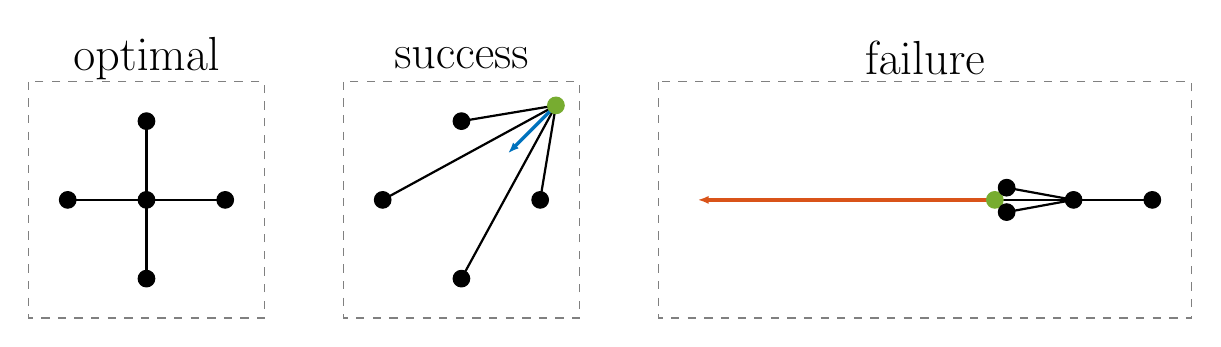
\begin{tikzpicture}
    \foreach \xA/\yA/\xB/\yB/\xC/\yC/\xD/\yD/\xE/\yE/\arrowX/\arrowY/\xShift/\xRect/\arrowV/\caZero/\caOne/\desc in {
        0/0/-1/0/0/1/0/-1/1/0/0/0/0/-1.5/a0/black/black/optimal,
        1.2/1.2/-1/0/0/1/0/-1/1/0/0.592271758813887/0.592271758813887/4/-1.5/a0/cC/black/success,
        0/0/-1/0/-0.85/0.155/-0.85/-0.155/1/0/-4.77422/0/11.77422/-5.27422/a1/black/cC/failure}{
        \begin{scope}[xshift=\xShift cm]
          \draw[dashed,color=gray,line width=0.5pt] (\xRect, 1.5) rectangle (1.5, -1.5);
          \node at ({(\xRect+1.5)/2}, 1.8) {\LARGE{\desc}};
          \coordinate (a0) at (\xA, \yA);
          \coordinate (a1) at (\xB, \yB);
          \coordinate (a2) at (\xC, \yC);
          \coordinate (a3) at (\xD, \yD);
          \coordinate (a4) at (\xE, \yE);
          \draw[thick] (a0) -- (a1);
          \draw[thick] (a0) -- (a2);
          \draw[thick] (a0) -- (a3);
          \draw[thick] (a0) -- (a4);

          \ifthenelse{\equal{\arrowX}{0} \AND \equal{\arrowY}{0}}{}{
          \ifthenelse{\equal{\desc}{success}}{
          \draw[-{Latex[length=4,width=3]},very thick,cA] (\arrowV) -- (\arrowX, \arrowY);
          }{
          \draw[-{Latex[length=4,width=3]},very thick,cD] (\arrowV) -- (\arrowX, \arrowY);
          }}

          \filldraw[draw=\caZero,fill=\caZero] (a0) circle (3pt);
          \filldraw[draw=\caOne,fill=\caOne]   (a1) circle (3pt);
          \filldraw[draw=black,fill=black] (a2) circle (3pt);
          \filldraw[draw=black,fill=black] (a3) circle (3pt);
          \filldraw[draw=black,fill=black] (a4) circle (3pt);
        \end{scope}
      }
  \end{tikzpicture}
  \caption{
    Visualization of the problem of the subspace method.
    Let a graph as shown in the left (optimal), where $k$ and all positive edge weights $w_{i,j}$ are set to 1.
    For the situation in the middle (success), the RSN works effectively.
    However, in the situation depicted on the right (failure),
    where the points are set as $x_0=(0,0), x_1=(-1,0), x_2=(-0.85,0.155), x_3=(-0.85,-0.155), x_4=(1,0)$,
    the Hessian for the subspace of $x_1$ is approximately
    $
      \begin{pmatrix} 1.841 & 0 \\ 0 & 1.159 \end{pmatrix}
    $.
    This Hessian, while positive definite and not ill-conditioned, leads to a Newton direction that clearly deviates significantly from the global optimal solution.
  }
  \label{fig:why_RSN_failed}
\end{figure*}

However, unfortunately, the RSN method is not necessarily effective for the FR layout.
As shown in Figure \ref{fig:why_RSN_failed}, although the energy function \( f_i \) with respect to the position \( x_i \) of each vertex is convex in the FR layout, the overall energy function \( f \) with respect to \( x_i \) is not convex.

これに対する解決策として、line searchの実施などである。しかし、そもそものNewton's directionが最適解から大きく外れるという問題は、必ずしも解決できない可能性があることには注意されたい。

\section{Another approach based on the Proposed Method}\label{sec:anotherApproach}

本論文では六方格子に基づいたSubspace Methodを提案したが、基本的に同一のアイデアに基づいた他のアプローチも考えられる。

\subsection{Non-randomized approach}\label{ssec:nonRandom}
一つは、各頂点毎に最適化する際に、ランダムに頂点を選んで最適化していくのではなく、$\abs{V}$点全てを同時に最適化する方法である。

こうすることによって、六方格子という制約をよりラフに扱うことが出来る。

六方格子への射影は、MinCostFlowなどで$\order{\abs{V}^3}$で厳密解が出せる。
ソートによる擬似的な射影で、$\order{\abs{V} \log \abs{V}}$で近似解が出せる。

\subsection{Non-Newton approach}\label{ssec:nonNewton}

もう一つは、Newton法を使わずに、勾配法を使う方法である。

以上のいずれも、基本的に性能は落ちると考えているが、実装が簡略化するなどの利点や、イテレーション毎の計算コストが多少減るという利点があり、検討の余地が残されている。

\end{document}